
%\section{User training}

Subjects were set to train their understanding of making distinguishable hand movements, using a user training interface, where feedback corresponding to the assigned group was presented. Prior to training subjects were informed of the importance of their efforts in relation to the experiment with the intent of encouraging a focused participation. \\
The user training interface contained the following feedback: an illustration of the movement needed to be performed, a horizontal bar visualizing the contraction level and a vertical bar plot visualizing which movement was being recognized by the control system. The only difference between the test and control group was the feedback received in the vertical bar plot. The test group received confidence score feedback (multiple bars) as seen in \figref{fig:test} and the control group received label feedback (single bar) as seen in \figref{fig:control}.

%\begin{figure}[H] 
%	\centering
%	\subfigure[Test group user training interface.]
%	{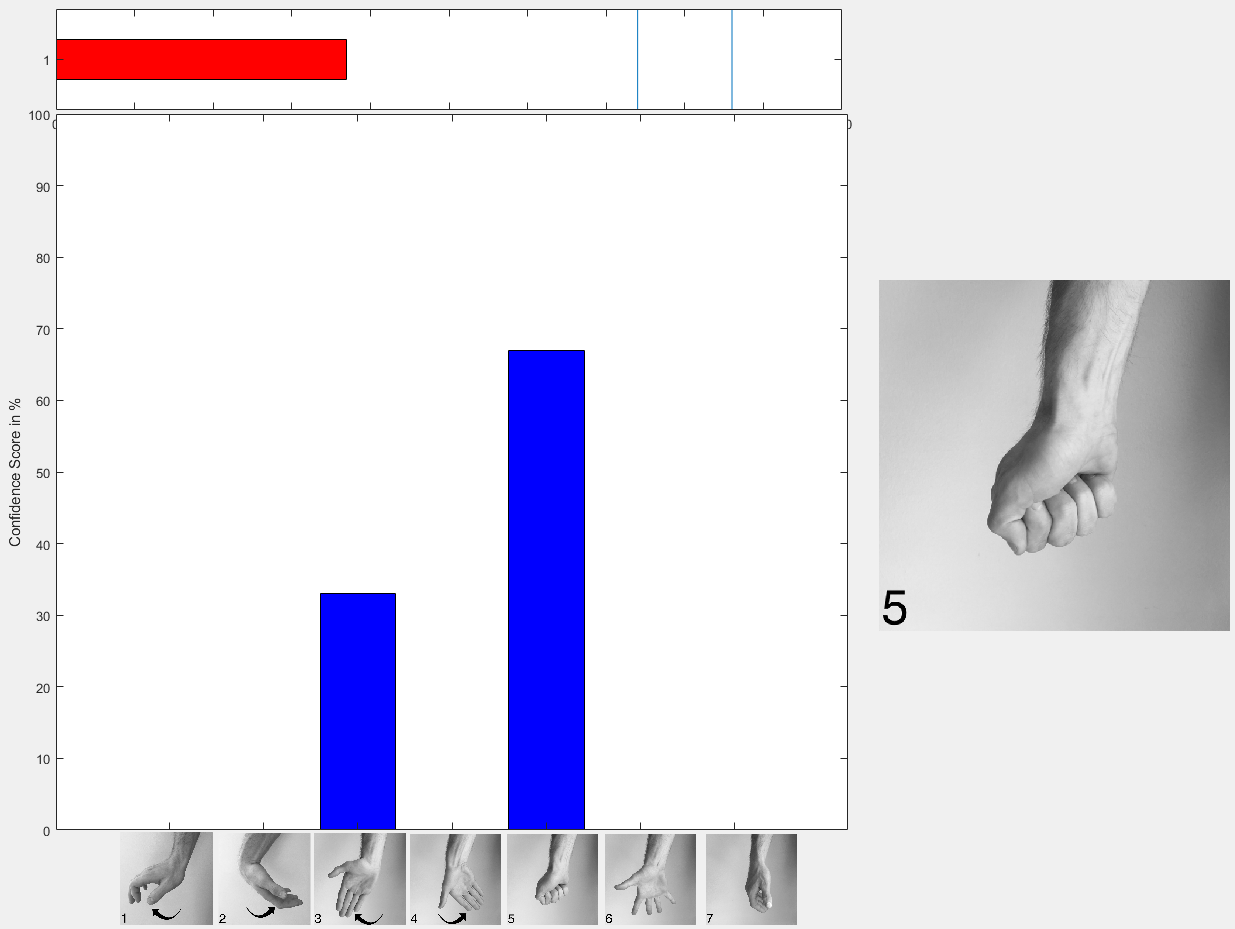
\includegraphics[width=.42\textwidth]{figures/xBackground/usertraintestGUI}} \\
%	\subfigure[Control group user training interface.]
%	{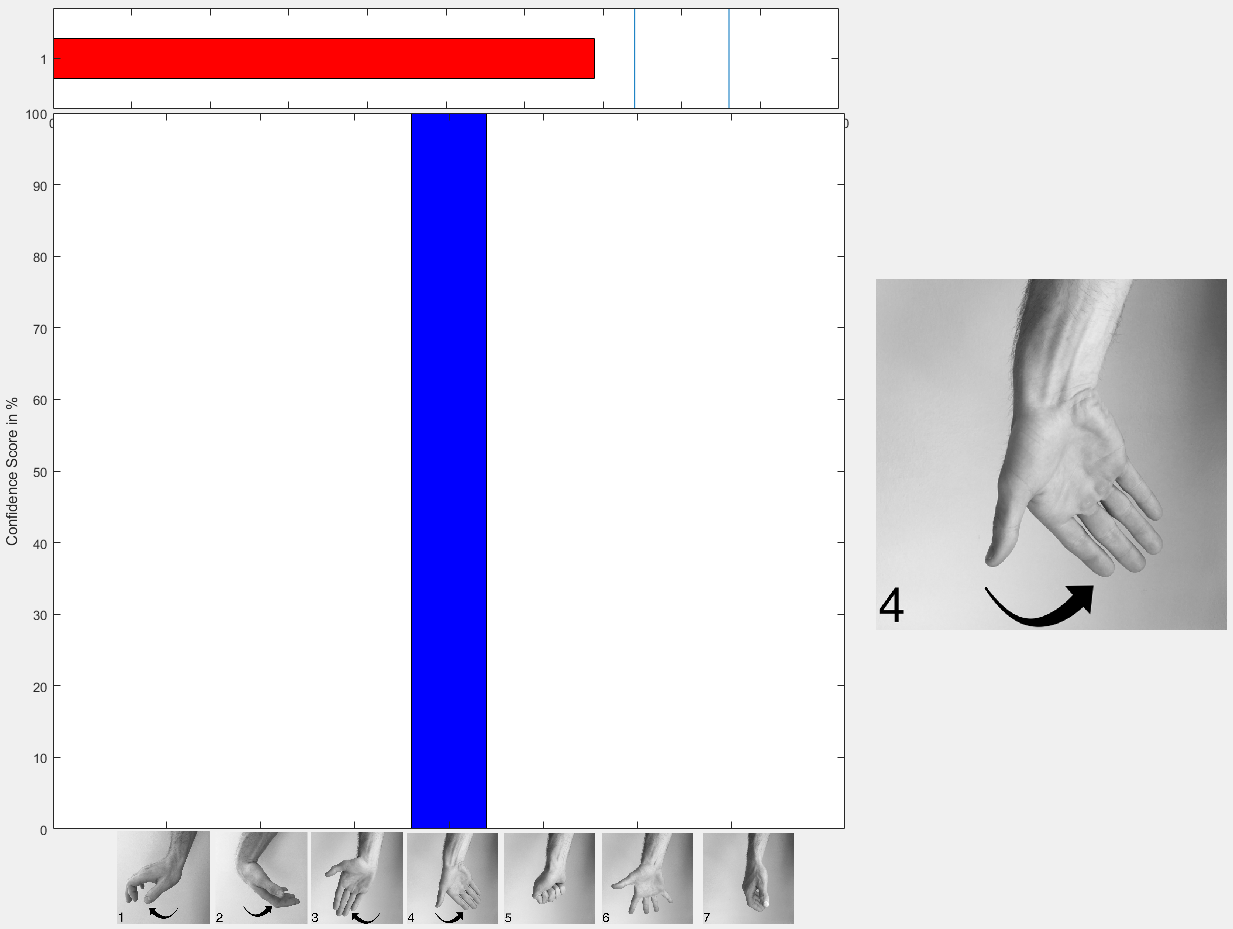
\includegraphics[width=.42\textwidth]{figures/xBackground/usertraincontrolGUI}}  
%	\caption{Illustration of the user training interface for the test group (a) and the control group (b). The vertical bar plot indicates which movement is being recognized visualized by the images of each movement; a full bar corresponds to 100 \% recognition confidence. The horizontal bar plot indicates contraction level, where a full bar corresponds to the MVC. The two vertical lines in the contraction level bar plot illustrates the contraction level interval the subject must reach. The large picture of a movement on the right of the bar plot indicates which movement needs to be performed. The difference between the feedback the two subject groups receive is the information given in the vertical recognition bar plot. The control group only sees a full bar of the movement the control system recognizes the most, whereas the test groups receives the exact recognition probabilities of all movements.}
%	\label{fig:feedbackGUI}
%\end{figure}


The test group was shown the classifier confidence scores for multiple classes, which enabled the possibility of having multiple vertical plots shown. Thus, more diverse feedback was presented, which the user could utilize to correct the performed movement. The control group had only the movement with the highest confidence shown, thereby limiting the confidence feedback to only one bar visible at a time. Thus, the control group was not informed on the exact probabilities of which movements the control system recognized.  

\begin{figure}[H]
	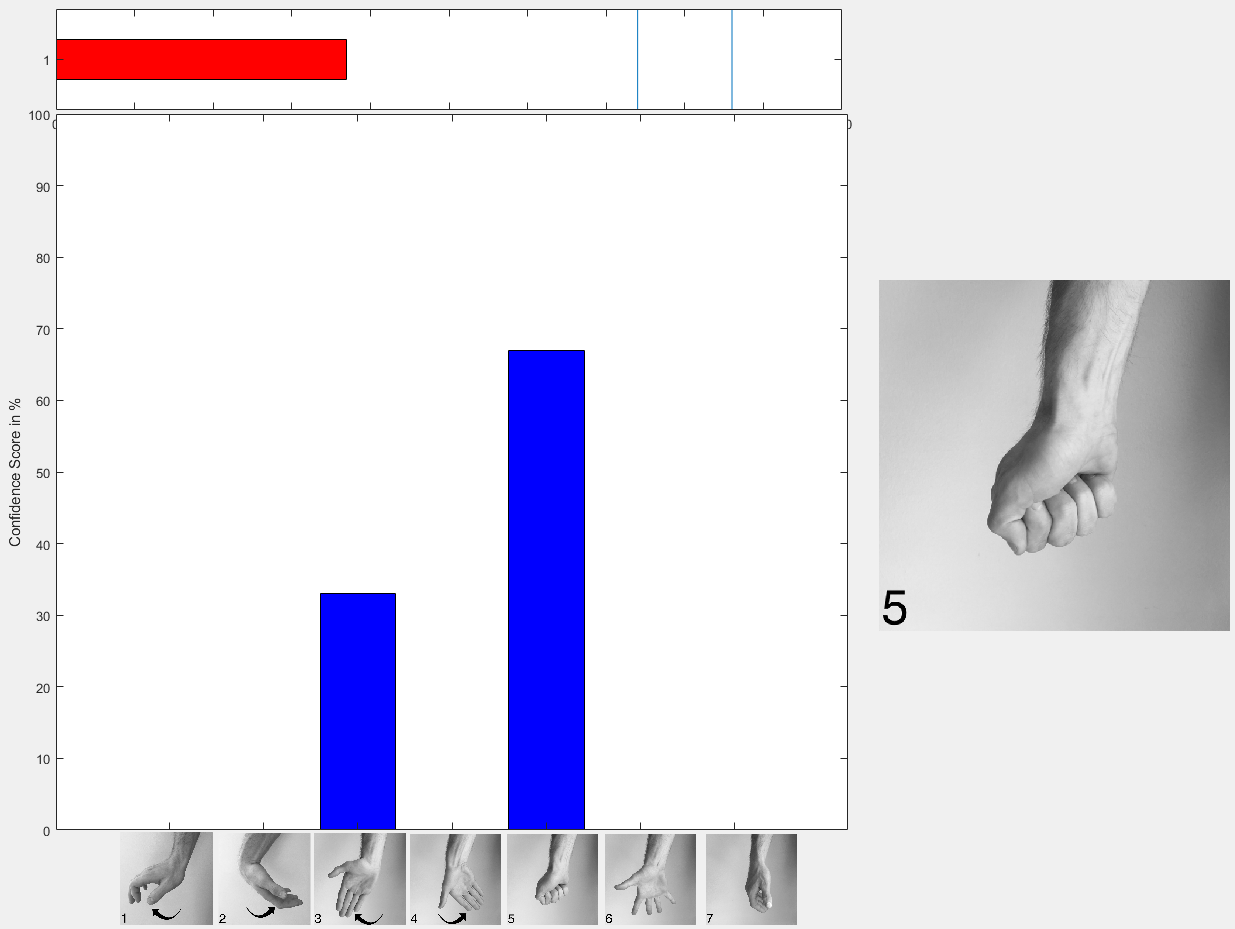
\includegraphics[width=.47\textwidth]{figures/xBackground/usertraintestGUI} \\
	\caption{Illustration of the user training interface for the test group. The vertical bar plot indicates which movement is being recognized visualized by the images of each movement; a full bar corresponds to 100 \% recognition confidence. The horizontal bar plot indicates contraction level, where a full bar corresponds to the MVC. The two vertical lines in the contraction level bar plot illustrates the contraction level interval the subject must reach. The large picture of a movement on the right of the bar plot indicates which movement needs to be performed. The test group received confidence score feedback by having the possibility of multiple bars being shown.}
	\label{fig:test}
\end{figure}    


The intent of user training was to train the subject in being more aware of how to perform a movement in a way the classifier would recognize as the movement the user actually performed. Basically, the training should motivate the subjects to modulate their contractions to maximize the classifier confidence. The subjects should perform contractions such that the probability bar for the target class is maximized while the probability bars for the other classes are minimized. To motivate the subject during user training a simple task was implemented in the interface. The subject had to perform the instructed movement and achieve a minimum of 75 \% confidence for the test group and the correct class for the control group, whilst also managing to perform the movement within the contraction level interval indicated by the vertical boundaries in the horizontal bar plot. Once these requirements were met and withheld for one second, a sound would appear indicating task completion. The subjects had to return to the rest class and then repeat the movement. A task completion was referred to as a repetition and was saved as a user training outcome measure. The goal was to manage as many repetitions as possible within 30 seconds, then a 10 second break was issued before moving to the next movement. \\
The sequence of a training session were put together in form of the subject having to perform each of the six movements in combination with four different contraction level intervals; 75-85 \%, 55-65 \%, 35-45 \% and 15-25 \% of their MVC. The instructed movements were trained in a random order and the subjects needed to perform all movements in the same contraction level interval before moving to a new interval. This resulted in a total training session time of 16 minutes.  

\begin{figure}[H]
	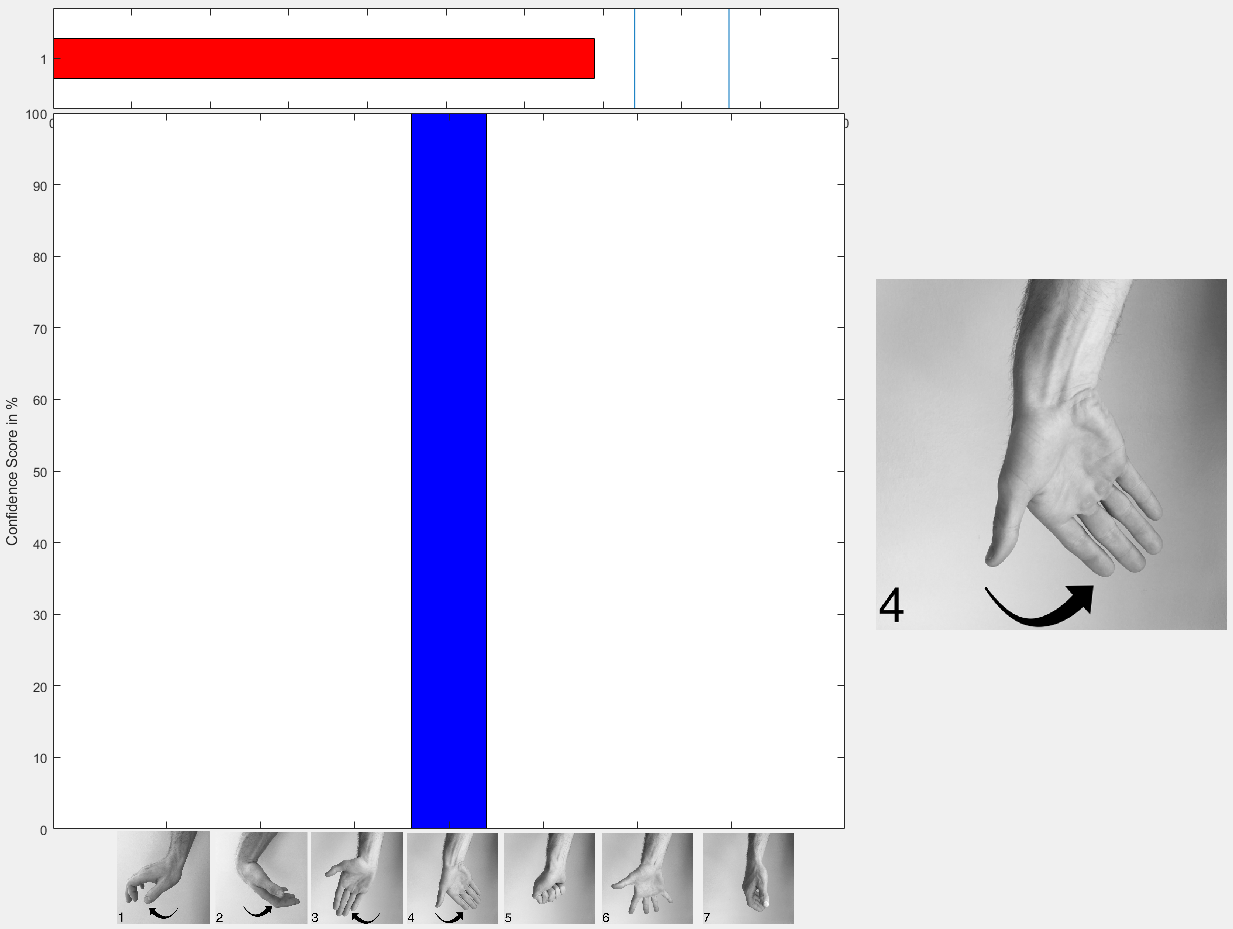
\includegraphics[width=.47\textwidth]{figures/xBackground/usertraincontrolGUI} \\
	\caption{Illustration of the user training interface for the control group. The same interface used for the test group was presented to the control group, except the feedback instead consisted of label feedback. Thereby the control group were only presented with the most certain recognized movement, shown with a single bar.}
	\label{fig:control}
\end{figure}       


